\documentclass[a4paper, 12pt]{article}
\usepackage[a4paper,top=1.5cm, bottom=1.5cm, left=1cm, right=1cm]{geometry}
\usepackage{cmap}					% поиск в PDF
\usepackage{mathtext} 				% русские буквы в формулах
\usepackage[T2A]{fontenc}			% кодировка
\usepackage[utf8]{inputenc}			% кодировка исходного текста
\usepackage[english,russian]{babel}	% локализация и переносы

\usepackage{amsmath,amssymb}
\usepackage{indentfirst}
\usepackage{longtable}
\usepackage{graphicx}
\usepackage{array}

\usepackage{wrapfig}
\usepackage{siunitx} % Required for alignment
\usepackage{subfigure}
\usepackage{multirow}
\usepackage{rotating}
\usepackage{caption}

\graphicspath{{.}}


\title{\begin{center}Лабораторная работа №3.1.3\end{center}
Измерение магнитного поля Земли}
\author{Рожков А. В.}
\date{\today}

\begin{document}
    \pagenumbering{gobble}
    \maketitle
    \newpage
    \pagenumbering{arabic}

    \textbf{Цель работы:} определить характеристики шарообразных неодимовых магнитов и, используя законы взаимодействия магнитных моментов с полем, измерить горизонтальную и вертикальную составляющие индукции магнитного поля Земли и магнитное наклонение.

	\textbf{В работе используются:} 12 одинаковых неодимовых магнитных шариков, тонкая нить для изготовления крутильного маятника, медная проволока диаметром (0,5 – 0,6) мм, электронные весы, секундомер, измеритель магнитной индукции АТЕ-8702, штангенциркуль, штатив из немагнитного материала, приспособление для определения расстояния действия магнитов; дополнительные неодимовые магнитные шарики ($\sim$20 шт.) и неодимовые магниты в форме параллелепипедов (2 шт.), набор гирь и разновесов.

    \section{Теория}
        \subsection{Точечный магнитный диполь}
            Простейший магнитный диполь может быть образован витком с током или постоянным магнитом. По определению, магнитный момент $\overrightarrow{P_m}$ тонкого витка площадью $S$ с током $I$ равен

            $$
            \overrightarrow{P_m}=\dfrac{I}{c}\vec{S}=\dfrac{I}{c}S\vec{n},
            $$
            где $\vec{S}=S\vec{n}$ -- вектор площади круга контура. Если размеры контура с током или магнитной стрелки малы по сравнению расстоянием до диполя, то соответствующий магнитный диполь называют элементарным или точечным.

            Магнитное поле точечного диполя определяется по формуле, аналогичной формуле для поля элементарного электрического диполя:

            $$
            \vec{B}=\dfrac{3(\overrightarrow{P_m},\vec{r})\vec{r}}{r^5} - \dfrac{\overrightarrow{P_m}}{r^3}
            $$

            В магнитном поле с индукцией $B$ на точечный магнитный диполь действует механический момент сил:

            $$
            \vec{M} = \overrightarrow{P_m}\times \vec{B}.
            $$

            Под действием вращающего момента $\vec{M}$ виток с током или постоянный магнит поворачивается так, чтобы его магнитный момент выстроился вдоль вектора индукции магнитного поля. Это — положение устойчивого равновесия: при отклонении от этого положения возникает механический момент внешних сил, возвращающий диполь к положению равновесия. В положении, когда $\overrightarrow{P_m}$ и $\vec{B}$ параллельны, но направлены противоположно друг другу, также имеет место равновесие ($M$ = 0), но такое равновесие неустойчиво: малейшее отклонение от этого положения приведёт к появлению момента сил, стремящихся отклонить диполь ещё дальше от начального положения.

            Магнитный диполь в магнитном поле обладает энергией:

            $$
            W = -(\overrightarrow{P_m},\vec{B})
            $$

            В неоднородном поле на точечный магнитный диполь, кроме момента сил, действует ещё и сила:

            $$
            \vec{F}=(\overrightarrow{P_m},\vec{\triangledown})\vec{B}
            $$

            Используя формулы для момента силы, силы и энергии, не сложно выяснить, как ведёт себя свободный магнитный диполь в неоднородном магнитном поле: он выстраивается вдоль силовых линий магнитного поля и, кроме того, под действием результирующей силы, возникающей из-за неоднородности поля, втягивается в область более сильного магнитного поля, т.е. в область, где он обладает меньшей энергией.

            Зная магнитные моменты $P_1 = P_2 = P_m$ двух небольших постоянных магнитов, можно рассчитать силу их взаимодействия:

            $$
            F = P_m \dfrac{\partial B}{\partial r}=-6\dfrac{P_m^2}{r^4}.
            $$

        \subsection{Неодимовые магнитные шары}
            В настоящей работе используются неодимовые магниты шарообразной формы. Для нас важно то, что:

            1) шары намагничены однородно;

            2) вещество, из которого изготовлены магниты, является магнитожёстким материалом.

            Полный магнитный момент $\overrightarrow{P_m}$ постоянного магнита определяется намагниченностью $\overrightarrow{p_m}$ вещества, из которого он изготовлен. По определению, намагниченность – это магнитный момент единицы объёма. Для однородно намагниченного шара намагниченность равна:

            $$
            \overrightarrow{p_m}=\dfrac{\overrightarrow{P_m}}{V}.
            $$

            Намагниченность — важная характеристика вещества постоянных магнитов, определяющая, в частности, величину остаточной магнитной индукции $B_r = 4\pi p_m$. Индукция магнитного поля $\overrightarrow{B_p}$ на полюсах однородно намагниченного шара связана с величиной намагниченности и остаточной магнитной индукцией формулами

            $$
            \overrightarrow{B_p}=\dfrac{8\pi}{3}\overrightarrow{p_m}=\dfrac{2}{3}\overrightarrow{B_r}.
            $$

    \section{Ход работы}

        \subsection{Определение магнитного момента, намагниченности и остаточной магнитной индукции вещества магнитных шариков}
            \subsubsection*{\textbf{Метод A}}
            \subsubsection{Вес шариков}

                При помощи весов измерим вес 12 шариков.

                \begin{table}[!ht]
                    \centering
                    \begin{tabular}{|c|c|c|c|c|c|c|c|c|c|c|c|c|}
                        \hline

                        \# & 1 & 2 & 3 & 4 & 5 & 6 & 7 & 8 & 9 & 10 & 11 & 12\\ \hline
                        $m, г$ & 0.791 & 0.864 & 0.816 & 0.802 & 0.816 & 0.845 & 0.838 & 0.832 & 0.820 & 0.829 & 0.840 & 0.832\\ \hline

                    \end{tabular}
                    \caption{Вес шариков}
                    \label{table:weight}
                \end{table}

                Среднее значение: $\langle m \rangle = (0.827 \pm 0.006)~г$

            \subsubsection{Максимальное расстояние взаимного удержания шариков}

                Измерим максимальное расстояние взаимного удержания шариков. Для этого используем специальное приспособление, которое представляет собой две раздвижные площадки.

                \begin{table}[!ht]
                    \centering
                    \begin{tabular}{|c|c|c|c|c|c|c|c|c|c|c|c|}
                        \hline

                        \# & 1 - 2 & 2 - 3 & 3 - 4 & 4 - 5 & 5 - 6 & 6 - 7 & 7 - 8 & 8 - 9 & 9 - 10 & 10 - 11 & 11 - 12\\ \hline
                        $r_{max}, см$ & 2.46 & 2.73 & 2.69 & 2.64 & 2.69 & 2.69 & 2.69 & 2.69 & 2.39 & 2.39 & 2.65\\ \hline

                    \end{tabular}
                    \caption{Максимальное расстояние взаимного удержания шариков}
                    \label{table:r_max}
                \end{table}

                Среднее значение: $\langle r_{max} \rangle = (2.61 \pm 0.04)~см$

            \subsubsection{Величина магнитного момента шарика}

                Из формул $F = 6P_m^2 / r_{max}^4$ и $F = mg$ рассчитаем величину среднюю величину магнитного момента шариков $P_m$

                $$
                    P_m = \sqrt{\frac{m g r_{max}^4}{6}} = (79 \pm 2)~Эрг/Гс
                $$


            \subsubsection{Величина намагниченности материала шариков}

                $$
                    p_m = \frac{P_m}{V} = (740 \pm 30)~Гс
                $$

            \subsubsection{Величина магнитного поля на полюсах шарика}

                Из величины магнитного момента шарика определим величину магнитного поля на полюсах шарика:

                $$
                    B_{эксп} = \frac{2P}{r^3} = (6200 \pm 400)~ед. СГСЭ
                $$

                При помощи измерителя магнитной индукции АТЕ-8702 получим величину магнитной индукции шариков.

                \begin{table}[!ht]
                    \centering
                    \begin{tabular}{|c|c|c|c|c|c|c|c|c|c|c|c|c|}
                        \hline

                        \# & 1 & 2 & 3 & 4 & 5 & 6 & 7 & 8 & 9 & 10 & 11 & 12\\ \hline
                        $B, ед. СГСЭ$ & 3054 & 3207 & 3133 & 3070 & 2118 & 2874 & 3064 & 3076 & 3070 & 3049 & 2829 & 3085\\ \hline

                    \end{tabular}
                    \caption{Величина магнитной индукции шариков}
                    \label{table:B}
                \end{table}

                Среднее значение: $\langle B_{изм} \rangle = (2970 \pm 80)~ед. СГСЭ$

            \subsubsection{Величина остаточной магнитной индукции материала}

                $$
                    B_r = 4 \pi p_m = (9260 \pm 40)~Гс
                $$

                Табличное значение для соединения неодим-железо-бор составляет $B_r = 11500-14500~Гс$

            \subsubsection*{\textbf{Метод B}}
            \subsubsection{Минимальный необходимый вес для отрыва верхнего шарика в цепочке}

                Составим цепочку из 20-30 шариков и присоединим её к грузикам. Подберём минимальный вес системы цепочки с гирей, при котором она отрывается от верхнего шарика.

                $$
                    F_{min} = (465890 \pm 1)~дин
                $$

            \subsubsection{Сила сцепления двух шаров}

                По формуле определим силу сцепления двух шаров

                $$
                    F_0 = F_{min} / 1,08 = (431379.7 \pm 0.9)~дин
                $$

            \subsubsection{Магнитный момент шарика}

                $$
                    P_m = \sqrt{\frac{F_0 d^4}{6}} = (93 \pm 7)~Эрг/Гс
                $$

            \subsubsection{Величина поля на полюсах}

                $$
                    B_{эксп} = \frac{2P}{r^3} = (7300 \pm 400)~ед. СГСЭ
                $$

                Напомним, что среднее измеренное при помощи магнетометра ATE-8702 значение составило $B_{изм} = (2970 \pm 80)~ед. СГСЭ$

            \subsubsection{Сравнение методов A и B}

                $$д
                    P_{m_A} = (79 \pm 2)~Эрг/Гс
                    P_{m_B} = (93 \pm 7)~Эрг/Гс
                $$

                Как видим, погрешность метода A меньше. Так же этот результат ближе к измеренному при помощи магнетометра ATE-8702

        \subsection{Определение горизонтальной составляющей магнитного поля Земли}

            \subsubsection{Юстировка системы из 12 шариков}

                Соберём цепочку из 12 шариков и произведём юстировку системы. Для этого распрямим цепочку и отрегулируем длину нитей $\Lambda$-образного подвеса для того, чтобы стрелка из шариков приняла горизонтальное положение.

            \subsubsection{Оценка влияния упругости нити на период крутильных колебаний}

                Свернём стрелку в окружность, чтобы исключить влияние магнитных полей. Оценим влияние упругости нити на период крутильных колебаний. Период одного колебания составил $T = 12,7~с$.  Это в 4 раза больше периода колебания прямой стрелки из 12 шариков ($12,7 / 3,11$). Период колебаний достаточно большой, чтобы пренебречь упругостью нити.

            \subsubsection{Зависимость периода крутильных колебаний "стрелки" от количества шариков в ней}

                Измерим период крутильных колебаний для разного количества шариков.

                \begin{table}[!ht]
                    \centering
                    \begin{tabular}{|c|c|c|c|c|c|c|c|}
                        \hline

                        $n, шт.$ & 4 & 5 & 6 & 7 & 8 & 10 & 12\\ \hline
                        $T, с$ & $1.31 \pm 0.03$ & $1.33 \pm 0.03$ & $1.86 \pm 0.03$ & $1.94 \pm 0.03$ & $2.16 \pm 0.03$ & $2.87 \pm 0.03$ & $3.11 \pm 0.03$\\ \hline

                    \end{tabular}
                    \caption{Результаты измерения периода крутильных колебаний горизонтальной стрелки}
                    \label{table:arrow_horizontal}
                \end{table}

                Для каждого количества шариков производилось измерение 10 колебаний. В таблице представлен период одного колебания.

            \subsubsection{График зависимости $T(n)$}

                При помощи МНК построим график

                \begin{figure}[!ht]
                    \centering
                    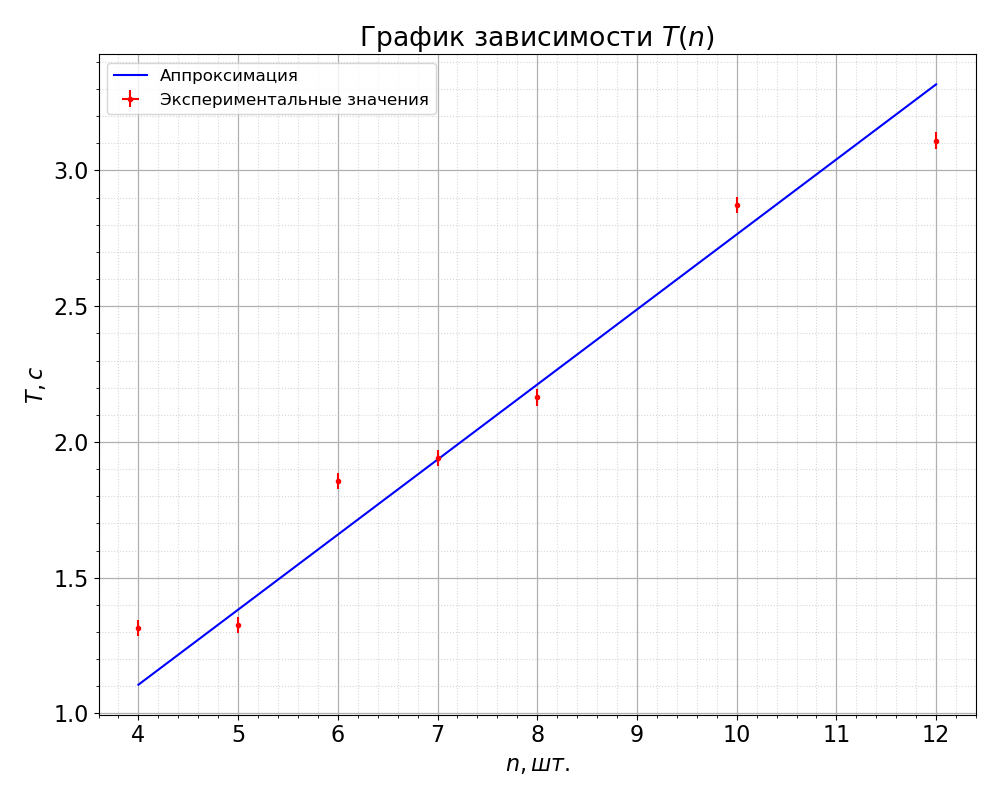
\includegraphics[width=0.75\textwidth]{img/horizontal.png}
                    \caption{График зависимости $T(n)$}
                    \label{plot:n_T_horizontal}
                \end{figure}

                $$
                    k = (0.276 \pm 0.07)~с
                $$

            \subsubsection{Величина горизонтальной составляющей магнитного поля Земли}

                $$
                    B_h = \frac{\pi^2md^2}{3k^2P_m} = (0.156 \pm 0.010)~Гс
                $$

        \subsection{Определение вертикальной составляющей магнитного поля Земли}

            \subsubsection{Момент сил, действующий со стороны магнитного Поля Земли на "стрелку" из нескольких шариков}

                \begin{table}[!ht]
                    \centering
                    \begin{tabular}{|c|c|c|c|c|c|}
                        \hline

                        $n, шт.$ & 4 & 6 & 8 & 10 & 12\\ \hline
                        $m, г$ & $0.372 \pm 0.001$ & $0.240 \pm 0.001$ & $0.158 \pm 0.001$ & $0.158 \pm 0.001$ & $0.218 \pm 0.001$\\ \hline
                        $M, г*см$ & $215 \pm 4$ & $278 \pm 5$ & $274 \pm 5$ & $365 \pm 7$ & $630 \pm 10$\\ \hline

                    \end{tabular}
                    \caption{Результаты измерения масс грузиков и моментов сил для уравновешивания вертикальной стрелки}
                    \label{table:arrow_vertical}
                \end{table}

            \subsubsection{График экспериментальной зависимости $M = M(n)$}

                \begin{figure}[!ht]
                    \centering
                    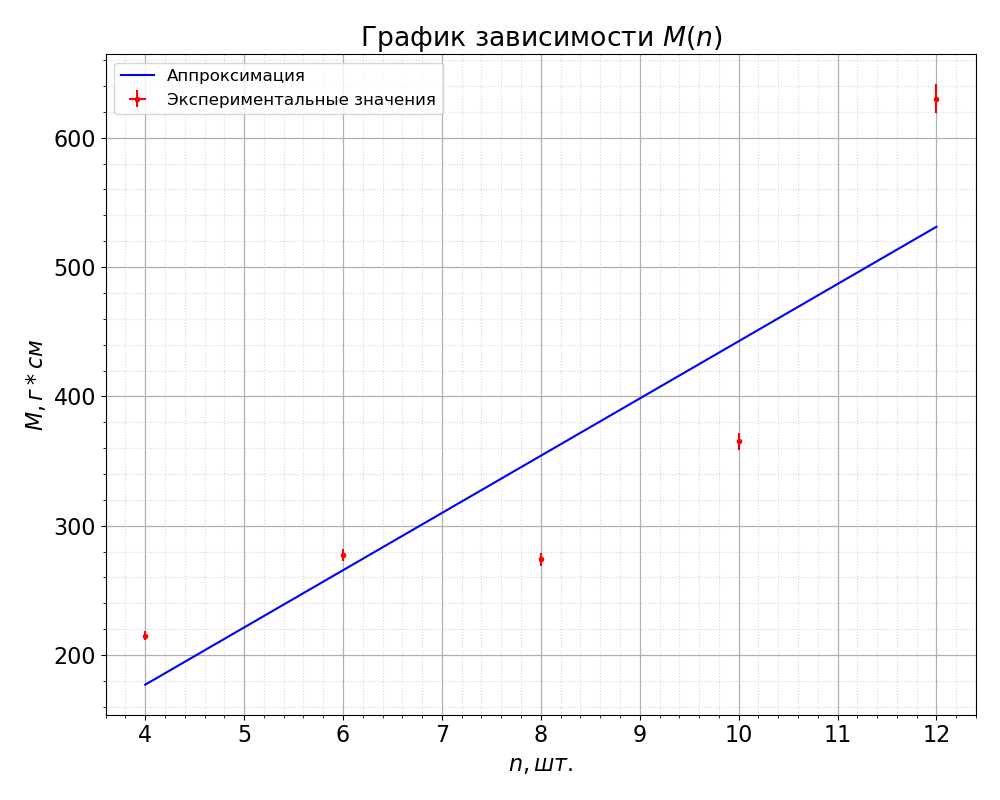
\includegraphics[width=0.75\textwidth]{img/vertical.png}
                    \caption{График зависимости $M(n)$}
                    \label{plot:n_M_vertical}
                \end{figure}

            \subsubsection{Аппроксимация экспериментальной зависимости}

                $$
                    k = (44 \pm 4)~г*см/с
                $$

            \subsubsection{Вертикальная составляющая магнитного поля Земли}

            \subsubsection{Полная величина индукции магнитного поля Земли}

            \subsubsection{Сравнение полученного результата со справочными данными}

\end{document}
